\documentclass[../dissertation.tex]{subfiles}

\begin{document}

\subsection{Experiment 6 - WiFi Connection (Real Data)}

This experiment was a repeat of Experiment 4, except using realistic data. The data used was the same MIT Stata Center dataset used previously in Experiment 5.

The aim of this experiment was to verify the results of Experiment 4 were valid when using common message types. The two message types used were sensor data, and video data, as discussed previously.

Expectations from this experiment were that the results of Experiment 4 would be exacerbated. The higher latencies of wifi would be exaggerated by using larger message sizes, and performance would degrade even faster than in Experiment 4.

\subsubsection{Results}

Results showed what has been classified as `good' performance at only 200Hz (see Figure \ref{exp6-sensor-wifi-all-freq-stream}). Raising the message frequency to 400Hz (and higher) introduced a significant drop in performance - from an average message latency of 23.1ms at 200Hz to 726.4ms at 400Hz, and peaking with a latency of 1721.4ms at 2000Hz (see Figure \ref{exp6-sensor-wifi-all-freq-mean}).

This leads to the conclusion that WiFi is a suitable choice of communication medium, as long as suitable low message frequency is chosen so as to ensure consistent performance. There was notable difference in performance at 200Hz from ethernet (23.1ms for WiFi, compared to 4.3ms for ethernet), however as the difference was consistent throughout the message stream (see Figure \ref{exp6-sensor-wifi-all-freq-stream}) this difference can be taken in to account for future experiments.

\begin{figure}[H]
\centering
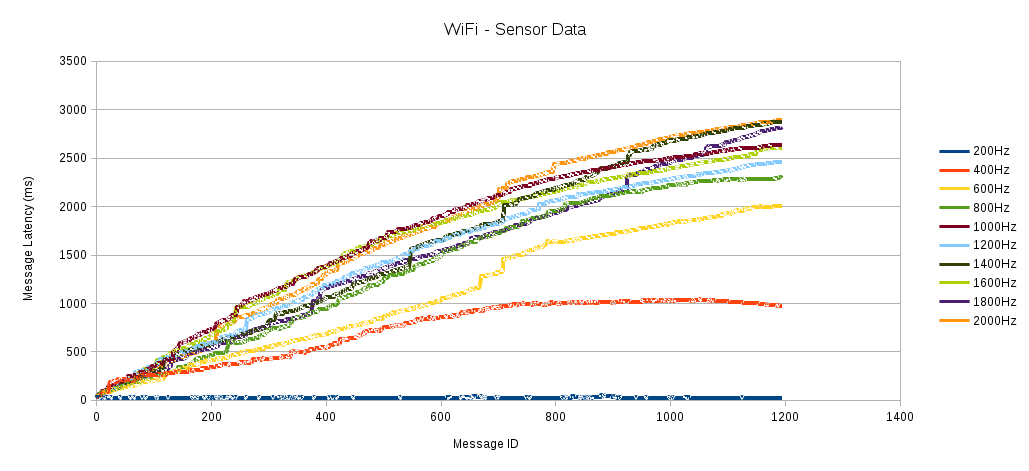
\includegraphics[width=\textwidth]{images/experiment6/sensor_data_wifi_all_freqs_stream.png}
\caption{Experiment 6 - Sensor Data WiFi, All Frequencies}
\label{exp6-sensor-wifi-all-freq-stream}
\end{figure}

\begin{figure}[H]
\centering
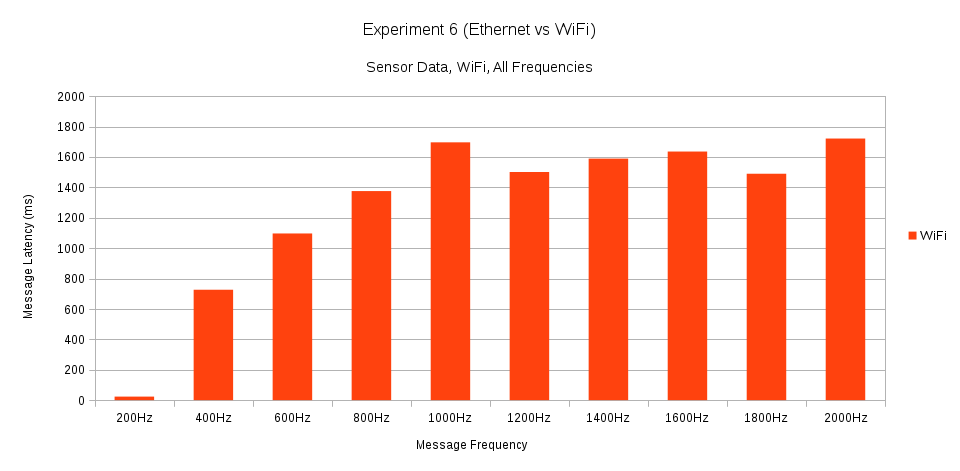
\includegraphics[width=\textwidth]{images/experiment6/sensor_data_wifi_all_freqs_mean.png}
\caption{Experiment 6 - Sensor Data WiFi, All Frequencies}
\label{exp6-sensor-wifi-all-freq-mean}
\end{figure}

\subsubsection{Further Investigation}

After the results shown in Figure \ref{exp6-sensor-wifi-all-freq-mean} demonstrated a significant difference between message frequencies of 200Hz and 400Hz, it was decided that further runs should be conducted between these frequencies to investigate the point at which performance degrades.

The extra runs conducted started at 100Hz (to gain information about performance below 200Hz), and increased in 50Hz increments up to 600Hz. The main areas of interest were 250Hz, 300Hz, and 350Hz.

As Figure \ref{exp6-sensor-wifi-more-freq-stream} shows, message stream performance was similar as seen before. Certain streams exhibited consistent low latency throughout their streams, but above a certain frequency (350Hz and up in this case) performance begins to degrade.

Figure \ref{exp6-sensor-wifi-more-freq-means} more clearly shows the jump in average message latency between 300Hz and 350Hz. This leads to the conclusion that for the sensor data message size (around 108kB), a suitable maximum frequency for publishing to ROS topics would be 300Hz.

\begin{figure}[H]
\centering
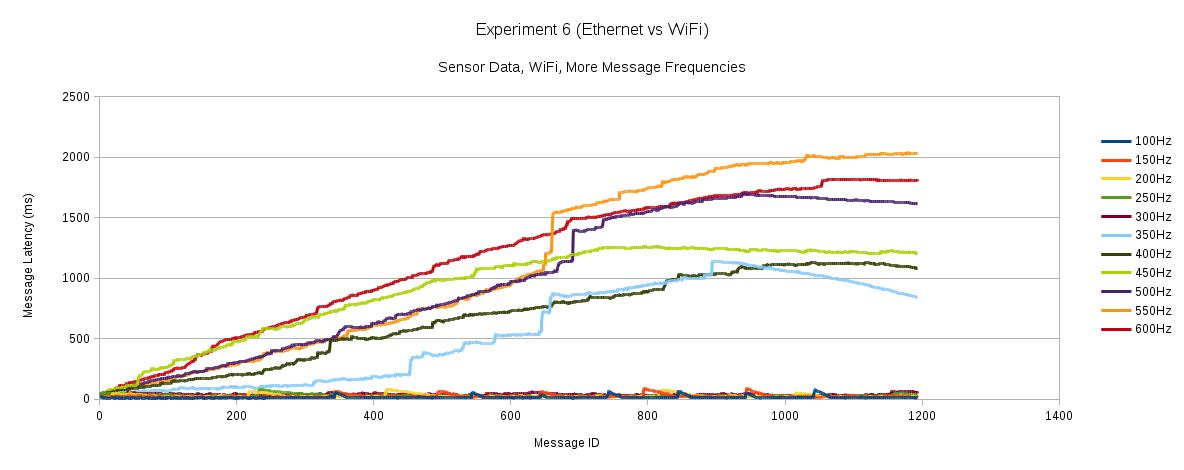
\includegraphics[width=\textwidth]{images/experiment6/sensor_data_wifi_more_freqs_stream.png}
\caption{Experiment 6 - Sensor Data WiFi, More Frequencies}
\label{exp6-sensor-wifi-more-freq-stream}
\end{figure}

\begin{figure}[H]
\centering
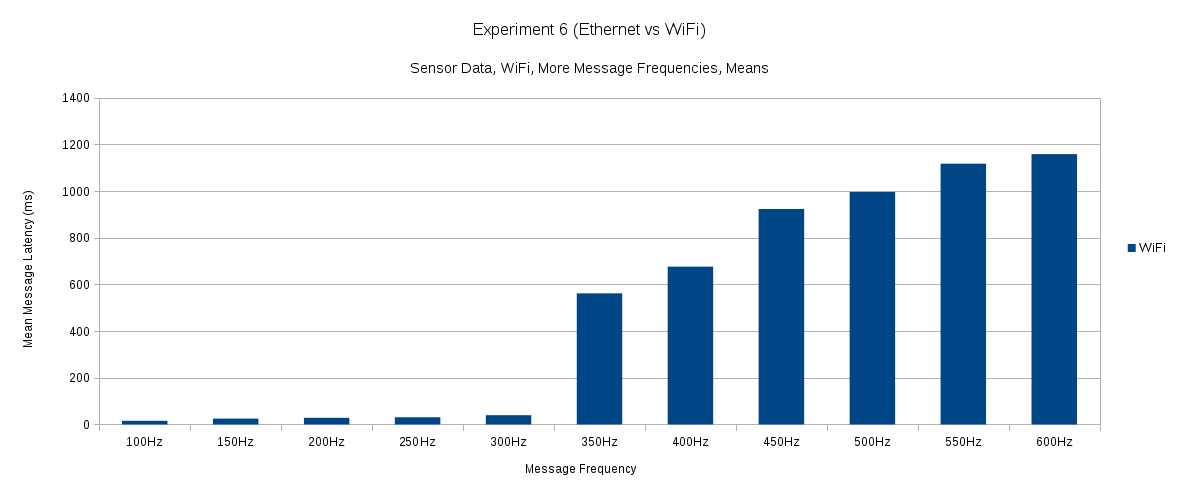
\includegraphics[width=\textwidth]{images/experiment6/sensor_data_wifi_more_freqs_means.png}
\caption{Experiment 6 - Sensor Data WiFi, More Frequencies}
\label{exp6-sensor-wifi-more-freq-means}
\end{figure}


\end{document}
